\documentclass[11pt,class=report,crop=false]{standalone}
\usepackage[screen]{../python}

\begin{document}

%====================================================================
\chapitre{Text viewer -- Markdown}
%====================================================================


\objectifs{You will program a simple word processor that displays paragraphs cleanly and highlights words in bold and italics.}

%%%%%%%%%%%%%%%%%%%%%%%%%%%%%%%%%%%%%%%%%%%%%%%%%%%%%%%%%%%%%%%%
%%%%%%%%%%%%%%%%%%%%%%%%%%%%%%%%%%%%%%%%%%%%%%%%%%%%%%%%%%%%%%%%

\begin{cours}[Text with tkinter]
Here's how to display text with \Python{} and the graphics window module 
\ci{tkinter}.

\index{module!tkinter@\ci{tkinter}}
\index{tkinter@\ci{tkinter}}

\begin{center}

\includegraphics[scale=0.6]{screen-markdown-7-en}
\end{center}
The code is:
\begin{lstlisting}
from tkinter import *
from tkinter.font import Font
# tkinter window
root = Tk()  
canvas = Canvas(root, width=800, height=600, background="white")
canvas.pack(fill="both", expand=True)
# Font
myfont = Font(family="Times", size=30)
# Some text
canvas.create_text(100,100, text="Text with Python!", 
anchor=SW, font=myfont, fill="blue")
# Launch the window
root.mainloop()
\end{lstlisting}


Some explanations:
\begin{itemize}
  \item \ci{root} and \ci{canvas} are the variables that define a graphic window (here of width $800$ and height $600$ pixels). This window is launched by the last command: \ci{root.mainloop()}.
  
  \item We remind you that for the graphic coordinates, the $y$-axis is directed downwards and the origin is the top-left corner. To define a rectangle, simply specify the coordinates $(x_1,y_1)$ and $(x_2,y_2)$ from two opposite vertices (see figure below). 
  
  \item The text is displayed by the \ci{canvas.create_text()} command. It is necessary to specify the coordinates $(x,y)$ of the point from which you want to display the text. 
  
  \item The \ci{text} option allows you to pass the string to display.
  
  \item The \ci{anchor} option allows you to specify the text anchor point, \ci{anchor=SW} means that the text box is anchored to the Southwest point (\emph{SW}) (see figure below).
  
  \item The \ci{fill} option allows you to specify the text color.
  
  \item The option \ci{font} allows you to define the font\index{font} (i.e. the style and size of the characters). Here are some examples of fonts, it's up to you to test them:
  \begin{itemize}
    \item \ci{Font(family="Times", size=20)} 
    \item \ci{Font(family="Courier", size=16, weight="bold")} in \textbf{bold}
    \item \ci{Font(family="Helvetica", size=16, slant="italic")} in \emph{italics}
  \end{itemize}  
\end{itemize}

\myfigure{0.7}{
\tikzinput{screen-markdown-8-en}
}


\end{cours}


%%%%%%%%%%%%%%%%%%%%%%%%%%%%%%%%%%%%%%%%%%%%%%%%%%%%%%%%%%%%%%%%
% Activity 1
%%%%%%%%%%%%%%%%%%%%%%%%%%%%%%%%%%%%%%%%%%%%%%%%%%%%%%%%%%%%%%%%

\begin{activite}[Display a text with tkinter]

\objectifs{Goal: display text with the graphics module \ci{tkinter}.}

\begin{center}
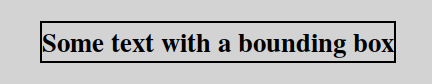
\includegraphics[scale=0.6]{screen-markdown-2-en}
\end{center}

\begin{enumerate}
  \item 
  \begin{enumerate}
    \item Define a \ci{tkinter} window of size $800 \times 600$ for example.

    \item Draw a gray rectangle (which will be our background box) with a size of \ci{back_width} $\times$ \ci{back_height} (for example $700 \times 500$).

    \item Define several types of fonts: \ci{title_font}, \ci{subtitle_font}, \ci{bold_font}, \ci{italic_font}, \ci{text_font}.
    
    \item Display texts with different fonts.
  \end{enumerate}
    
  \item Write a \ci{text_box(word,font)} function that draws a rectangle around a text. To do this, use the \ci{canvas.bbox(myobject)} method which returns the $x_1,y_1,x_2,y_2$ coordinates of the desired rectangle. (Here \ci{myobject = canvas.create_text(...)}).
  
  \item Write a \ci{length_word(word,font)} function that calculates the length of a word in pixels (this is the width of the rectangle from the previous question).
  
  \item Write a \ci{font_choice(mode,in_bold,in_italics)} function that returns the name of an adapted font (among those defined in the first question) according to a mode (among \ci{"title"}, \ci{"subtitle"}, \ci{"text"}) and according to booleans \ci{in_bold}, \ci{in_italics}.
  
  For example, \ci{font_choice("text",True,False)} returns the font \ci{bold_font}.
\end{enumerate}

\end{activite}


%%%%%%%%%%%%%%%%%%%%%%%%%%%%%%%%%%%%%%%%%%%%%%%%%%%%%%%%%%%%%%%%
%%%%%%%%%%%%%%%%%%%%%%%%%%%%%%%%%%%%%%%%%%%%%%%%%%%%%%%%%%%%%%%%

\begin{cours}[Markdown]
The \emph{Markdown}\index{markdown@\emph{markdown}} is a simple markup language that allows you to write your own easy to read text file and possibly convert it to another format (html, pdf\ldots).

Here is an example of a text file with the \emph{Markdown} syntax with its graphic rendering just below.
\begin{center}
\footnotesize
\begin{minipage}{0.7\textwidth}
\begin{verbatim}
# On the Origins of Species

## by Charles Darwin

When on board H.M.S. * Beagle * as naturalist, I was much struck with 
certain facts in the distribution of the inhabitants of South America, 
and in the geological relations of the present to the past inhabitants 
of that continent. These facts seemed to me to throw some light on the 
** origin of species ** that mystery of mysteries, as it has been called 
by one of our greatest philosophers.

## Chapters

+ Variation under domestication.
+ Variation under nature.
+ Struggle for existence.
+ Natural selection. 
+ ...
\end{verbatim}
\end{minipage}
\end{center}
\begin{center}
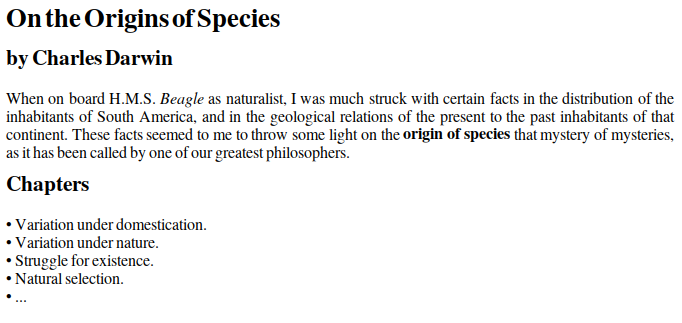
\includegraphics[scale=0.6]{screen-markdown-1-en}
\end{center}


The syntax is simple, with a clear and clean text file. Here are some elements of this syntax:
\begin{itemize}
  \item a \textbf{bold text} is obtained by surrounding the text with two asterisks \ci{**};
  \item a \emph{text in italics} is obtained by surrounding the text with one asterisk \ci{*};
  \item the line of a title begins with one hashtag \#;
  \item the line of a subtitle begins with two hashtags \#\#;
  \item for the elements of a list, each line starts with a special symbol, for us it will be the \og{}plus\fg{} symbol \ci{+}.
  \item There is also syntax to display links, tables, code\ldots 
\end{itemize}

In the following we will use the simplified syntax as described above.
\end{cours}

%%%%%%%%%%%%%%%%%%%%%%%%%%%%%%%%%%%%%%%%%%%%%%%%%%%%%%%%%%%%%%%%
% Activity 2
%%%%%%%%%%%%%%%%%%%%%%%%%%%%%%%%%%%%%%%%%%%%%%%%%%%%%%%%%%%%%%%%

\begin{activite}[View \emph{Markdown}]

\objectifs{Goal: display text with our simplified \emph{Markdown} syntax.}

\begin{enumerate}
  \item Write a function \ci{print_line_v1(par,posy)} that displays \emph{one by one} the words of a paragraph \ci{par} (at the line of ordinate \ci{posy}). 
  
\begin{center}
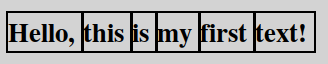
\includegraphics[scale=0.6]{screen-markdown-3-en}
\end{center}   

  \emph{Hints.}
  \begin{itemize}
    \item These words are obtained one by one with the command \ci{par.split()}.
    \item The displayed line starts at the very left, it overflows to the right if it is too long.
    \item After each word we place a space and then the next word.
    \item In the picture above the words are framed.
   \end{itemize}
   
 
  \item Improve your function in \ci{print_line_v2(par,posy)} to take into account titles, subtitles and lists.
  
   
\begin{center}
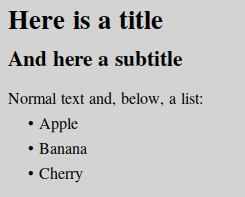
\includegraphics[scale=0.7]{screen-markdown-4-en}
\end{center}    
  
  \emph{Hints.}
    \begin{itemize}
    \item To know which mode to use when displaying the line, simply test the first characters of the line. The line of a title begins with \#, that of a subtitle with \#\#, that of a list with \ci{+}. 
    
    \item For lists, you can get the bullet point character \og{}\textbullet\fg{} by the unicode character \ci{u'\\u2022'}\index{unicode}. You can also indent each item of the list for more readability.
    
    \item Use the \ci{font_choice()} function from the first activity.
    
    \item In the image above, each line is produced by a call to the function. For example \ci{print_line_v2("## And here a subtitle",100)}.
   \end{itemize}


  \item Further improve your function in \ci{print_line_v3(par,posy)} to take into account the words in bold and italics in the text.
  
\begin{center}
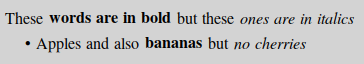
\includegraphics[scale=0.7]{screen-markdown-5-en}
\end{center}   
 
 	\emph{Hints.}
  \begin{itemize}
    \item Words in bold are surrounded by the tag \ci{**}, words in italics by the tag \ci{*}. In our simplified syntax, tags are separated from words by spaces, for example: \lstinline!"Words ** in bold ** and in * italics *"!
    
    
    \item Define a boolean variable \ci{in_bold} that is false at the beginning; each time you encounter the tag \ci{**} reverse the value of \ci{in_bold} (\og{}True\fg{} becomes \og{}False\fg{}, \og{}False\fg{} becomes \og{}True\fg{}, you can use the \ci{not} operator).
    
    \item Still use the \ci{font_choice()} function from the first activity.
    
    \item In the image above, each line is produced by a call to the function. For example \ci{print_line_v3("+ Apples and also ** bananas ** but * no cherries *",100)}
   \end{itemize} 
   
   
  \item Further improve your function in \ci{print_paragraph(par,posy)} which manages the display of a paragraph (i.e. a string that can be very long) on several lines.
  
\begin{center}
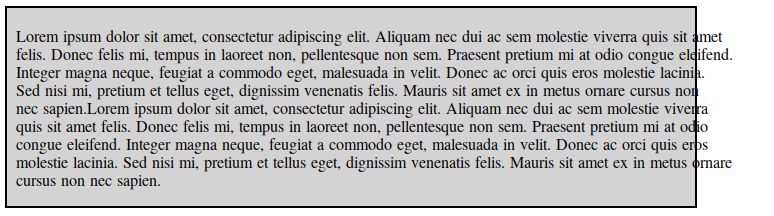
\includegraphics[scale=0.55]{screen-markdown-6-en}
\end{center}   
 
   \emph{Hints.}
  \begin{itemize}
    \item As soon as you place a word that exceeds the length of the line (see those that come out of the frame in the image above), then the next word is placed on the next line.
    
    \item The function will therefore modify the variable \ci{posy} at each line break. At the end, the function returns the new value of \ci{posy}, which will be useful for displaying the next paragraph.
 
   \end{itemize}    
   
   \item End with a \ci{print_file(filename)} function that displays the paragraphs of a text file with our simplified \emph{Markdown} syntax.
\end{enumerate} 
\end{activite}

%%%%%%%%%%%%%%%%%%%%%%%%%%%%%%%%%%%%%%%%%%%%%%%%%%%%%%%%%%%%%%%%
% Activity 3
%%%%%%%%%%%%%%%%%%%%%%%%%%%%%%%%%%%%%%%%%%%%%%%%%%%%%%%%%%%%%%%%

\begin{activite}[Justification]

\objectifs{Goal: understand how it is possible to \og{}justify\fg{} a text, i.e. to ensure that the words are well aligned on the left and right sides of the page. To model the problem we work with a series of integers that represent the lengths of our words.}


In this activity:
\begin{itemize}
 \item \ci{list_lengths} is a list of integers (for example a list of $50$ integers between $5$ and $15$) which represent the lengths of the words;
 \item we set a constant \ci{line_length} which represents the length of a line. For our examples, this length is equal to $100$.
 \end{itemize}


In previous activities, we moved to the next line after a word had passed the end of the line.
We represent this by the following figure:
\begin{center}
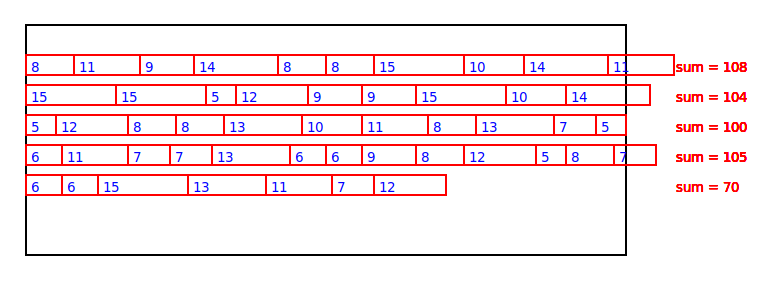
\includegraphics[scale=0.5]{screen-hyphen-1}
\end{center} 
You're going to try to place the words more nicely!

The drawings are based on the example:
\begin{center}
\ci{list_lengths =} [8, 11, 9, 14, 8, 8, 15, 10, 14, 11, 15, 15, 5, 12, 9, 9, 15, 10, 14, 5, 12, 8, 8, 13, 10, 11, 8, 13, 7, 5, 6, 11, 7, 7, 13, 6, 6, 9, 8, 12, 5, 8, 7, 6, 6, 15, 13, 11, 7, 12]
\end{center}
which was obtained by random integers:
\begin{lstlisting}
from random import randint
list_lengths = [randint(5,15) for i in range(50)]
\end{lstlisting}


\begin{enumerate}
  \item Write a \ci{justification_simple()} function that calculates the indices at which to make the text alignment corresponding to the figure below, i.e. an alignment on the left (without spaces) and without exceeding the total length of the line (here of length $100$).
  
\begin{center}
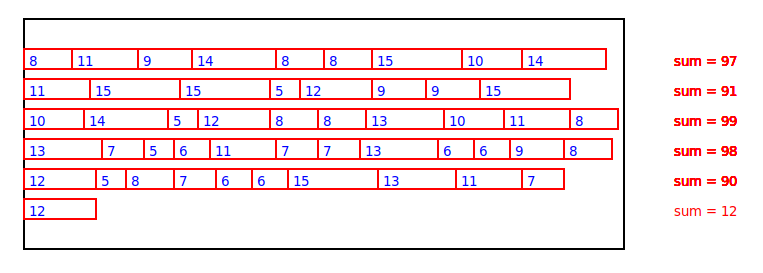
\includegraphics[scale=0.5]{screen-hyphen-2}
\end{center} 

  \begin{fonction}[\ci{justification_simple()}]
  Use: \ci{justification_simple(list_lengths)} \\
  Input: a sequence of lengths (a list of integers)\\
  Output: the list of indices where to make a cut
  \medskip
    
  Example: \ci{justification_simple(list_lengths)} where \ci{list_lengths} is the example given above, returns the list \ci{[0, 9, 17, 27, 39, 49, 50]}. That is to say that:
  \begin{itemize}
    \item the first line corresponds to indices $0$ to $8$ (given by \ci{range(0,9)}),
    \item the second line corresponds to indices $9$ to $16$ (given by \ci{range(9,17)}),
    \item the third line corresponds to indices $17$ to $26$ (given by \ci{range(17,27)}),
    \item \ldots
    \item the last line corresponds to the index $49$ (given by \ci{range(49,50)}).
    \end{itemize}
             
  \end{fonction}

  \item Modify your work into a \ci{justification_spaces()} function that adds a space (with \ci{space_length = 1}) between two words of the same line (but not at the beginning of the line, nor at the end of the line). This corresponds to the following drawing:
  
\begin{center}
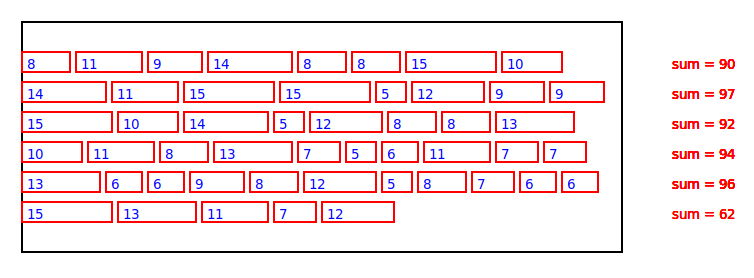
\includegraphics[scale=0.5]{screen-hyphen-3}
\end{center} 

For our example, the justifications returned are \ci{[0, 8, 16, 24, 34, 45, 50]}.


  \item In order to be able to justify the text, you allow spaces to be larger than the initial length of $1$. On each line, the spaces between the words are all the same length (greater than or equal to $1$) so that the last word is aligned on the right. From one line to another, the length of the spaces can change.
 
\begin{center}
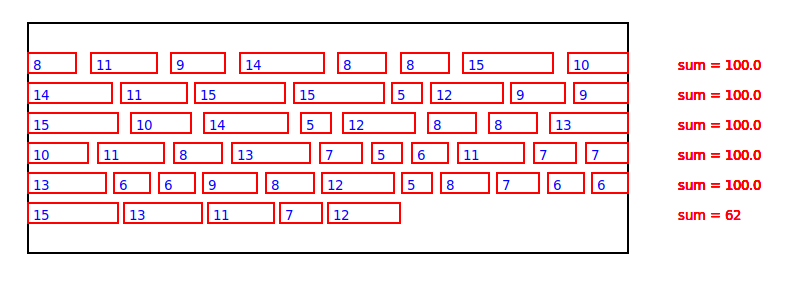
\includegraphics[scale=0.5]{screen-hyphen-4}
\end{center}

Write a \ci{compute_space_lengths()} function that returns the length that the spaces of each line must have in order for the text to be justified.
For our example, we obtain the list \ci{[2.43, 1.43, 2.14, 1.67, 1.40, 1.00]}, i.e. for the first line the spaces must be $2.43$ long, for the second line $1.43$,\ldots 

To find the right formula, simply take the results of the \ci{justification_spaces()} function and then, for each line, count the total length of words it contains, as well as the value it lacks to arrive at a total of $100$.
\end{enumerate} 
\end{activite}


\bigskip
\bigskip

\objectifs{You now have everything you need to visualize text written with the \emph{Markdown} syntax and justify it (see Darwin's text displayed text in the lesson). It's still a lot of work! You can also improve the support of the \emph{Markdown} syntax: code, numbered lists, sublists, bold and italic words at the same time\ldots}


\end{document}
